% Created by tikzDevice version 0.12.6 on 2024-04-17 08:44:32
% !TEX encoding = UTF-8 Unicode
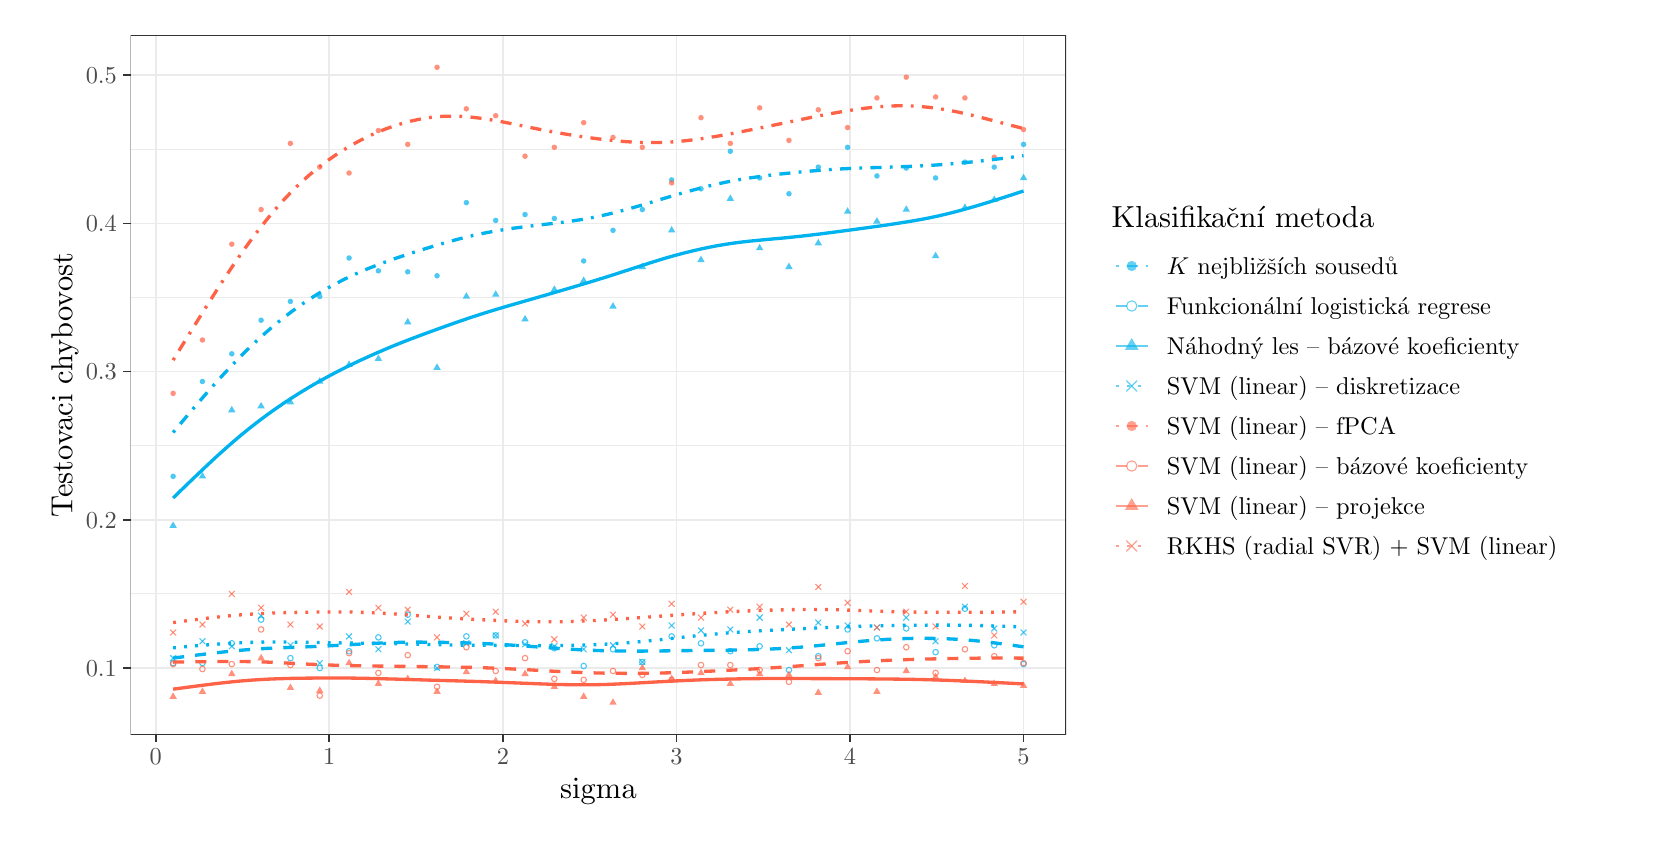
\begin{tikzpicture}[x=1pt,y=1pt]
\definecolor{fillColor}{RGB}{255,255,255}
\path[use as bounding box,fill=fillColor] (0,0) rectangle (578.16,289.08);
\begin{scope}
\path[clip] (  0.00,  0.00) rectangle (578.16,289.08);
\definecolor{drawColor}{RGB}{255,255,255}

\path[draw=drawColor,line width= 0.6pt,line join=round,line cap=round,fill=fillColor] (  0.00,  0.00) rectangle (578.16,289.08);
\end{scope}
\begin{scope}
\path[clip] ( 37.19, 33.72) rectangle (375.23,286.23);
\definecolor{fillColor}{RGB}{255,255,255}

\path[fill=fillColor] ( 37.19, 33.72) rectangle (375.23,286.23);
\definecolor{drawColor}{gray}{0.92}

\path[draw=drawColor,line width= 0.3pt,line join=round] ( 37.19, 84.47) --
	(375.23, 84.47);

\path[draw=drawColor,line width= 0.3pt,line join=round] ( 37.19,138.02) --
	(375.23,138.02);

\path[draw=drawColor,line width= 0.3pt,line join=round] ( 37.19,191.57) --
	(375.23,191.57);

\path[draw=drawColor,line width= 0.3pt,line join=round] ( 37.19,245.13) --
	(375.23,245.13);

\path[draw=drawColor,line width= 0.6pt,line join=round] ( 37.19, 57.69) --
	(375.23, 57.69);

\path[draw=drawColor,line width= 0.6pt,line join=round] ( 37.19,111.25) --
	(375.23,111.25);

\path[draw=drawColor,line width= 0.6pt,line join=round] ( 37.19,164.80) --
	(375.23,164.80);

\path[draw=drawColor,line width= 0.6pt,line join=round] ( 37.19,218.35) --
	(375.23,218.35);

\path[draw=drawColor,line width= 0.6pt,line join=round] ( 37.19,271.90) --
	(375.23,271.90);

\path[draw=drawColor,line width= 0.6pt,line join=round] ( 46.29, 33.72) --
	( 46.29,286.23);

\path[draw=drawColor,line width= 0.6pt,line join=round] (109.00, 33.72) --
	(109.00,286.23);

\path[draw=drawColor,line width= 0.6pt,line join=round] (171.72, 33.72) --
	(171.72,286.23);

\path[draw=drawColor,line width= 0.6pt,line join=round] (234.43, 33.72) --
	(234.43,286.23);

\path[draw=drawColor,line width= 0.6pt,line join=round] (297.15, 33.72) --
	(297.15,286.23);

\path[draw=drawColor,line width= 0.6pt,line join=round] (359.86, 33.72) --
	(359.86,286.23);
\definecolor{fillColor}{RGB}{0,178,238}

\path[fill=fillColor,fill opacity=0.70] ( 52.56,126.95) circle (  1.00);

\path[fill=fillColor,fill opacity=0.70] ( 63.15,161.23) circle (  1.00);

\path[fill=fillColor,fill opacity=0.70] ( 73.75,171.22) circle (  1.00);

\path[fill=fillColor,fill opacity=0.70] ( 84.35,183.36) circle (  1.00);

\path[fill=fillColor,fill opacity=0.70] ( 94.94,190.15) circle (  1.00);

\path[fill=fillColor,fill opacity=0.70] (105.54,191.93) circle (  1.00);

\path[fill=fillColor,fill opacity=0.70] (116.14,205.85) circle (  1.00);

\path[fill=fillColor,fill opacity=0.70] (126.73,201.21) circle (  1.00);

\path[fill=fillColor,fill opacity=0.70] (137.33,200.86) circle (  1.00);

\path[fill=fillColor,fill opacity=0.70] (147.93,199.43) circle (  1.00);

\path[fill=fillColor,fill opacity=0.70] (158.52,225.85) circle (  1.00);

\path[fill=fillColor,fill opacity=0.70] (169.12,219.42) circle (  1.00);

\path[fill=fillColor,fill opacity=0.70] (179.72,221.56) circle (  1.00);

\path[fill=fillColor,fill opacity=0.70] (190.31,220.13) circle (  1.00);

\path[fill=fillColor,fill opacity=0.70] (200.91,204.78) circle (  1.00);

\path[fill=fillColor,fill opacity=0.70] (211.51,215.85) circle (  1.00);

\path[fill=fillColor,fill opacity=0.70] (222.10,223.35) circle (  1.00);

\path[fill=fillColor,fill opacity=0.70] (232.70,234.06) circle (  1.00);

\path[fill=fillColor,fill opacity=0.70] (243.30,230.84) circle (  1.00);

\path[fill=fillColor,fill opacity=0.70] (253.90,244.41) circle (  1.00);

\path[fill=fillColor,fill opacity=0.70] (264.49,234.77) circle (  1.00);

\path[fill=fillColor,fill opacity=0.70] (275.09,229.06) circle (  1.00);

\path[fill=fillColor,fill opacity=0.70] (285.69,238.70) circle (  1.00);

\path[fill=fillColor,fill opacity=0.70] (296.28,245.84) circle (  1.00);

\path[fill=fillColor,fill opacity=0.70] (306.88,235.49) circle (  1.00);

\path[fill=fillColor,fill opacity=0.70] (317.48,238.34) circle (  1.00);

\path[fill=fillColor,fill opacity=0.70] (328.07,234.77) circle (  1.00);

\path[fill=fillColor,fill opacity=0.70] (338.67,240.48) circle (  1.00);

\path[fill=fillColor,fill opacity=0.70] (349.27,238.70) circle (  1.00);

\path[fill=fillColor,fill opacity=0.70] (359.86,246.91) circle (  1.00);
\definecolor{drawColor}{RGB}{0,178,238}

\path[draw=drawColor,draw opacity=0.70,line width= 0.4pt,line join=round,line cap=round] ( 52.56, 59.48) circle (  1.00);

\path[draw=drawColor,draw opacity=0.70,line width= 0.4pt,line join=round,line cap=round] ( 63.15, 59.48) circle (  1.00);

\path[draw=drawColor,draw opacity=0.70,line width= 0.4pt,line join=round,line cap=round] ( 73.75, 66.62) circle (  1.00);

\path[draw=drawColor,draw opacity=0.70,line width= 0.4pt,line join=round,line cap=round] ( 84.35, 75.19) circle (  1.00);

\path[draw=drawColor,draw opacity=0.70,line width= 0.4pt,line join=round,line cap=round] ( 94.94, 61.26) circle (  1.00);

\path[draw=drawColor,draw opacity=0.70,line width= 0.4pt,line join=round,line cap=round] (105.54, 57.69) circle (  1.00);

\path[draw=drawColor,draw opacity=0.70,line width= 0.4pt,line join=round,line cap=round] (116.14, 63.76) circle (  1.00);

\path[draw=drawColor,draw opacity=0.70,line width= 0.4pt,line join=round,line cap=round] (126.73, 68.76) circle (  1.00);

\path[draw=drawColor,draw opacity=0.70,line width= 0.4pt,line join=round,line cap=round] (137.33, 76.97) circle (  1.00);

\path[draw=drawColor,draw opacity=0.70,line width= 0.4pt,line join=round,line cap=round] (147.93, 58.05) circle (  1.00);

\path[draw=drawColor,draw opacity=0.70,line width= 0.4pt,line join=round,line cap=round] (158.52, 69.12) circle (  1.00);

\path[draw=drawColor,draw opacity=0.70,line width= 0.4pt,line join=round,line cap=round] (169.12, 69.48) circle (  1.00);

\path[draw=drawColor,draw opacity=0.70,line width= 0.4pt,line join=round,line cap=round] (179.72, 66.98) circle (  1.00);

\path[draw=drawColor,draw opacity=0.70,line width= 0.4pt,line join=round,line cap=round] (190.31, 64.84) circle (  1.00);

\path[draw=drawColor,draw opacity=0.70,line width= 0.4pt,line join=round,line cap=round] (200.91, 58.41) circle (  1.00);

\path[draw=drawColor,draw opacity=0.70,line width= 0.4pt,line join=round,line cap=round] (211.51, 64.48) circle (  1.00);

\path[draw=drawColor,draw opacity=0.70,line width= 0.4pt,line join=round,line cap=round] (222.10, 59.84) circle (  1.00);

\path[draw=drawColor,draw opacity=0.70,line width= 0.4pt,line join=round,line cap=round] (232.70, 69.12) circle (  1.00);

\path[draw=drawColor,draw opacity=0.70,line width= 0.4pt,line join=round,line cap=round] (243.30, 66.62) circle (  1.00);

\path[draw=drawColor,draw opacity=0.70,line width= 0.4pt,line join=round,line cap=round] (253.90, 63.76) circle (  1.00);

\path[draw=drawColor,draw opacity=0.70,line width= 0.4pt,line join=round,line cap=round] (264.49, 65.55) circle (  1.00);

\path[draw=drawColor,draw opacity=0.70,line width= 0.4pt,line join=round,line cap=round] (275.09, 56.98) circle (  1.00);

\path[draw=drawColor,draw opacity=0.70,line width= 0.4pt,line join=round,line cap=round] (285.69, 61.98) circle (  1.00);

\path[draw=drawColor,draw opacity=0.70,line width= 0.4pt,line join=round,line cap=round] (296.28, 71.62) circle (  1.00);

\path[draw=drawColor,draw opacity=0.70,line width= 0.4pt,line join=round,line cap=round] (306.88, 68.41) circle (  1.00);

\path[draw=drawColor,draw opacity=0.70,line width= 0.4pt,line join=round,line cap=round] (317.48, 71.98) circle (  1.00);

\path[draw=drawColor,draw opacity=0.70,line width= 0.4pt,line join=round,line cap=round] (328.07, 63.41) circle (  1.00);

\path[draw=drawColor,draw opacity=0.70,line width= 0.4pt,line join=round,line cap=round] (338.67, 79.12) circle (  1.00);

\path[draw=drawColor,draw opacity=0.70,line width= 0.4pt,line join=round,line cap=round] (349.27, 65.91) circle (  1.00);

\path[draw=drawColor,draw opacity=0.70,line width= 0.4pt,line join=round,line cap=round] (359.86, 59.12) circle (  1.00);

\path[fill=fillColor,fill opacity=0.70] ( 52.56,110.66) --
	( 53.90,108.33) --
	( 51.21,108.33) --
	cycle;

\path[fill=fillColor,fill opacity=0.70] ( 63.15,128.51) --
	( 64.50,126.18) --
	( 61.81,126.18) --
	cycle;

\path[fill=fillColor,fill opacity=0.70] ( 73.75,152.43) --
	( 75.10,150.10) --
	( 72.41,150.10) --
	cycle;

\path[fill=fillColor,fill opacity=0.70] ( 84.35,153.85) --
	( 85.69,151.53) --
	( 83.00,151.53) --
	cycle;

\path[fill=fillColor,fill opacity=0.70] ( 94.94,155.28) --
	( 96.29,152.95) --
	( 93.60,152.95) --
	cycle;

\path[fill=fillColor,fill opacity=0.70] (105.54,162.78) --
	(106.89,160.45) --
	(104.20,160.45) --
	cycle;

\path[fill=fillColor,fill opacity=0.70] (116.14,168.85) --
	(117.48,166.52) --
	(114.79,166.52) --
	cycle;

\path[fill=fillColor,fill opacity=0.70] (126.73,170.99) --
	(128.08,168.66) --
	(125.39,168.66) --
	cycle;

\path[fill=fillColor,fill opacity=0.70] (137.33,184.20) --
	(138.68,181.87) --
	(135.99,181.87) --
	cycle;

\path[fill=fillColor,fill opacity=0.70] (147.93,167.78) --
	(149.27,165.45) --
	(146.58,165.45) --
	cycle;

\path[fill=fillColor,fill opacity=0.70] (158.52,193.48) --
	(159.87,191.15) --
	(157.18,191.15) --
	cycle;

\path[fill=fillColor,fill opacity=0.70] (169.12,194.20) --
	(170.47,191.87) --
	(167.78,191.87) --
	cycle;

\path[fill=fillColor,fill opacity=0.70] (179.72,185.27) --
	(181.06,182.94) --
	(178.37,182.94) --
	cycle;

\path[fill=fillColor,fill opacity=0.70] (190.31,195.98) --
	(191.66,193.65) --
	(188.97,193.65) --
	cycle;

\path[fill=fillColor,fill opacity=0.70] (200.91,199.20) --
	(202.26,196.87) --
	(199.57,196.87) --
	cycle;

\path[fill=fillColor,fill opacity=0.70] (211.51,189.91) --
	(212.85,187.58) --
	(210.16,187.58) --
	cycle;

\path[fill=fillColor,fill opacity=0.70] (222.10,204.19) --
	(223.45,201.86) --
	(220.76,201.86) --
	cycle;

\path[fill=fillColor,fill opacity=0.70] (232.70,217.40) --
	(234.05,215.07) --
	(231.36,215.07) --
	cycle;

\path[fill=fillColor,fill opacity=0.70] (243.30,206.69) --
	(244.64,204.36) --
	(241.95,204.36) --
	cycle;

\path[fill=fillColor,fill opacity=0.70] (253.90,228.83) --
	(255.24,226.50) --
	(252.55,226.50) --
	cycle;

\path[fill=fillColor,fill opacity=0.70] (264.49,210.98) --
	(265.84,208.65) --
	(263.15,208.65) --
	cycle;

\path[fill=fillColor,fill opacity=0.70] (275.09,204.19) --
	(276.43,201.86) --
	(273.74,201.86) --
	cycle;

\path[fill=fillColor,fill opacity=0.70] (285.69,212.76) --
	(287.03,210.43) --
	(284.34,210.43) --
	cycle;

\path[fill=fillColor,fill opacity=0.70] (296.28,224.19) --
	(297.63,221.86) --
	(294.94,221.86) --
	cycle;

\path[fill=fillColor,fill opacity=0.70] (306.88,220.62) --
	(308.22,218.29) --
	(305.53,218.29) --
	cycle;

\path[fill=fillColor,fill opacity=0.70] (317.48,224.90) --
	(318.82,222.57) --
	(316.13,222.57) --
	cycle;

\path[fill=fillColor,fill opacity=0.70] (328.07,208.12) --
	(329.42,205.79) --
	(326.73,205.79) --
	cycle;

\path[fill=fillColor,fill opacity=0.70] (338.67,225.61) --
	(340.01,223.29) --
	(337.32,223.29) --
	cycle;

\path[fill=fillColor,fill opacity=0.70] (349.27,228.47) --
	(350.61,226.14) --
	(347.92,226.14) --
	cycle;

\path[fill=fillColor,fill opacity=0.70] (359.86,236.32) --
	(361.21,234.00) --
	(358.52,234.00) --
	cycle;

\path[draw=drawColor,draw opacity=0.70,line width= 0.4pt,line join=round,line cap=round] ( 51.56, 60.27) -- ( 53.56, 62.26);

\path[draw=drawColor,draw opacity=0.70,line width= 0.4pt,line join=round,line cap=round] ( 51.56, 62.26) -- ( 53.56, 60.27);

\path[draw=drawColor,draw opacity=0.70,line width= 0.4pt,line join=round,line cap=round] ( 62.16, 66.34) -- ( 64.15, 68.33);

\path[draw=drawColor,draw opacity=0.70,line width= 0.4pt,line join=round,line cap=round] ( 62.16, 68.33) -- ( 64.15, 66.34);

\path[draw=drawColor,draw opacity=0.70,line width= 0.4pt,line join=round,line cap=round] ( 72.75, 64.55) -- ( 74.75, 66.55);

\path[draw=drawColor,draw opacity=0.70,line width= 0.4pt,line join=round,line cap=round] ( 72.75, 66.55) -- ( 74.75, 64.55);

\path[draw=drawColor,draw opacity=0.70,line width= 0.4pt,line join=round,line cap=round] ( 83.35, 75.62) -- ( 85.35, 77.61);

\path[draw=drawColor,draw opacity=0.70,line width= 0.4pt,line join=round,line cap=round] ( 83.35, 77.61) -- ( 85.35, 75.62);

\path[draw=drawColor,draw opacity=0.70,line width= 0.4pt,line join=round,line cap=round] ( 93.95, 64.91) -- ( 95.94, 66.90);

\path[draw=drawColor,draw opacity=0.70,line width= 0.4pt,line join=round,line cap=round] ( 93.95, 66.90) -- ( 95.94, 64.91);

\path[draw=drawColor,draw opacity=0.70,line width= 0.4pt,line join=round,line cap=round] (104.54, 58.48) -- (106.54, 60.48);

\path[draw=drawColor,draw opacity=0.70,line width= 0.4pt,line join=round,line cap=round] (104.54, 60.48) -- (106.54, 58.48);

\path[draw=drawColor,draw opacity=0.70,line width= 0.4pt,line join=round,line cap=round] (115.14, 68.12) -- (117.14, 70.12);

\path[draw=drawColor,draw opacity=0.70,line width= 0.4pt,line join=round,line cap=round] (115.14, 70.12) -- (117.14, 68.12);

\path[draw=drawColor,draw opacity=0.70,line width= 0.4pt,line join=round,line cap=round] (125.74, 63.48) -- (127.73, 65.48);

\path[draw=drawColor,draw opacity=0.70,line width= 0.4pt,line join=round,line cap=round] (125.74, 65.48) -- (127.73, 63.48);

\path[draw=drawColor,draw opacity=0.70,line width= 0.4pt,line join=round,line cap=round] (136.33, 73.48) -- (138.33, 75.47);

\path[draw=drawColor,draw opacity=0.70,line width= 0.4pt,line join=round,line cap=round] (136.33, 75.47) -- (138.33, 73.48);

\path[draw=drawColor,draw opacity=0.70,line width= 0.4pt,line join=round,line cap=round] (146.93, 56.70) -- (148.93, 58.69);

\path[draw=drawColor,draw opacity=0.70,line width= 0.4pt,line join=round,line cap=round] (146.93, 58.69) -- (148.93, 56.70);

\path[draw=drawColor,draw opacity=0.70,line width= 0.4pt,line join=round,line cap=round] (157.53, 65.62) -- (159.52, 67.62);

\path[draw=drawColor,draw opacity=0.70,line width= 0.4pt,line join=round,line cap=round] (157.53, 67.62) -- (159.52, 65.62);

\path[draw=drawColor,draw opacity=0.70,line width= 0.4pt,line join=round,line cap=round] (168.12, 68.48) -- (170.12, 70.47);

\path[draw=drawColor,draw opacity=0.70,line width= 0.4pt,line join=round,line cap=round] (168.12, 70.47) -- (170.12, 68.48);

\path[draw=drawColor,draw opacity=0.70,line width= 0.4pt,line join=round,line cap=round] (178.72, 65.26) -- (180.72, 67.26);

\path[draw=drawColor,draw opacity=0.70,line width= 0.4pt,line join=round,line cap=round] (178.72, 67.26) -- (180.72, 65.26);

\path[draw=drawColor,draw opacity=0.70,line width= 0.4pt,line join=round,line cap=round] (189.32, 64.55) -- (191.31, 66.55);

\path[draw=drawColor,draw opacity=0.70,line width= 0.4pt,line join=round,line cap=round] (189.32, 66.55) -- (191.31, 64.55);

\path[draw=drawColor,draw opacity=0.70,line width= 0.4pt,line join=round,line cap=round] (199.91, 63.48) -- (201.91, 65.48);

\path[draw=drawColor,draw opacity=0.70,line width= 0.4pt,line join=round,line cap=round] (199.91, 65.48) -- (201.91, 63.48);

\path[draw=drawColor,draw opacity=0.70,line width= 0.4pt,line join=round,line cap=round] (210.51, 64.91) -- (212.51, 66.90);

\path[draw=drawColor,draw opacity=0.70,line width= 0.4pt,line join=round,line cap=round] (210.51, 66.90) -- (212.51, 64.91);

\path[draw=drawColor,draw opacity=0.70,line width= 0.4pt,line join=round,line cap=round] (221.11, 58.84) -- (223.10, 60.84);

\path[draw=drawColor,draw opacity=0.70,line width= 0.4pt,line join=round,line cap=round] (221.11, 60.84) -- (223.10, 58.84);

\path[draw=drawColor,draw opacity=0.70,line width= 0.4pt,line join=round,line cap=round] (231.70, 72.05) -- (233.70, 74.04);

\path[draw=drawColor,draw opacity=0.70,line width= 0.4pt,line join=round,line cap=round] (231.70, 74.04) -- (233.70, 72.05);

\path[draw=drawColor,draw opacity=0.70,line width= 0.4pt,line join=round,line cap=round] (242.30, 70.26) -- (244.30, 72.26);

\path[draw=drawColor,draw opacity=0.70,line width= 0.4pt,line join=round,line cap=round] (242.30, 72.26) -- (244.30, 70.26);

\path[draw=drawColor,draw opacity=0.70,line width= 0.4pt,line join=round,line cap=round] (252.90, 70.62) -- (254.89, 72.62);

\path[draw=drawColor,draw opacity=0.70,line width= 0.4pt,line join=round,line cap=round] (252.90, 72.62) -- (254.89, 70.62);

\path[draw=drawColor,draw opacity=0.70,line width= 0.4pt,line join=round,line cap=round] (263.49, 74.90) -- (265.49, 76.90);

\path[draw=drawColor,draw opacity=0.70,line width= 0.4pt,line join=round,line cap=round] (263.49, 76.90) -- (265.49, 74.90);

\path[draw=drawColor,draw opacity=0.70,line width= 0.4pt,line join=round,line cap=round] (274.09, 63.12) -- (276.09, 65.12);

\path[draw=drawColor,draw opacity=0.70,line width= 0.4pt,line join=round,line cap=round] (274.09, 65.12) -- (276.09, 63.12);

\path[draw=drawColor,draw opacity=0.70,line width= 0.4pt,line join=round,line cap=round] (284.69, 73.12) -- (286.68, 75.12);

\path[draw=drawColor,draw opacity=0.70,line width= 0.4pt,line join=round,line cap=round] (284.69, 75.12) -- (286.68, 73.12);

\path[draw=drawColor,draw opacity=0.70,line width= 0.4pt,line join=round,line cap=round] (295.28, 72.05) -- (297.28, 74.04);

\path[draw=drawColor,draw opacity=0.70,line width= 0.4pt,line join=round,line cap=round] (295.28, 74.04) -- (297.28, 72.05);

\path[draw=drawColor,draw opacity=0.70,line width= 0.4pt,line join=round,line cap=round] (305.88, 71.33) -- (307.88, 73.33);

\path[draw=drawColor,draw opacity=0.70,line width= 0.4pt,line join=round,line cap=round] (305.88, 73.33) -- (307.88, 71.33);

\path[draw=drawColor,draw opacity=0.70,line width= 0.4pt,line join=round,line cap=round] (316.48, 74.90) -- (318.47, 76.90);

\path[draw=drawColor,draw opacity=0.70,line width= 0.4pt,line join=round,line cap=round] (316.48, 76.90) -- (318.47, 74.90);

\path[draw=drawColor,draw opacity=0.70,line width= 0.4pt,line join=round,line cap=round] (327.07, 66.34) -- (329.07, 68.33);

\path[draw=drawColor,draw opacity=0.70,line width= 0.4pt,line join=round,line cap=round] (327.07, 68.33) -- (329.07, 66.34);

\path[draw=drawColor,draw opacity=0.70,line width= 0.4pt,line join=round,line cap=round] (337.67, 78.83) -- (339.67, 80.83);

\path[draw=drawColor,draw opacity=0.70,line width= 0.4pt,line join=round,line cap=round] (337.67, 80.83) -- (339.67, 78.83);

\path[draw=drawColor,draw opacity=0.70,line width= 0.4pt,line join=round,line cap=round] (348.27, 70.98) -- (350.26, 72.97);

\path[draw=drawColor,draw opacity=0.70,line width= 0.4pt,line join=round,line cap=round] (348.27, 72.97) -- (350.26, 70.98);

\path[draw=drawColor,draw opacity=0.70,line width= 0.4pt,line join=round,line cap=round] (358.86, 69.55) -- (360.86, 71.55);

\path[draw=drawColor,draw opacity=0.70,line width= 0.4pt,line join=round,line cap=round] (358.86, 71.55) -- (360.86, 69.55);
\definecolor{fillColor}{RGB}{255,99,71}

\path[fill=fillColor,fill opacity=0.70] ( 52.56,156.94) circle (  1.00);

\path[fill=fillColor,fill opacity=0.70] ( 63.15,176.22) circle (  1.00);

\path[fill=fillColor,fill opacity=0.70] ( 73.75,210.85) circle (  1.00);

\path[fill=fillColor,fill opacity=0.70] ( 84.35,223.35) circle (  1.00);

\path[fill=fillColor,fill opacity=0.70] ( 94.94,247.27) circle (  1.00);

\path[fill=fillColor,fill opacity=0.70] (105.54,238.70) circle (  1.00);

\path[fill=fillColor,fill opacity=0.70] (116.14,236.56) circle (  1.00);

\path[fill=fillColor,fill opacity=0.70] (126.73,251.91) circle (  1.00);

\path[fill=fillColor,fill opacity=0.70] (137.33,246.91) circle (  1.00);

\path[fill=fillColor,fill opacity=0.70] (147.93,274.76) circle (  1.00);

\path[fill=fillColor,fill opacity=0.70] (158.52,259.76) circle (  1.00);

\path[fill=fillColor,fill opacity=0.70] (169.12,257.26) circle (  1.00);

\path[fill=fillColor,fill opacity=0.70] (179.72,242.63) circle (  1.00);

\path[fill=fillColor,fill opacity=0.70] (190.31,245.84) circle (  1.00);

\path[fill=fillColor,fill opacity=0.70] (200.91,254.76) circle (  1.00);

\path[fill=fillColor,fill opacity=0.70] (211.51,249.41) circle (  1.00);

\path[fill=fillColor,fill opacity=0.70] (222.10,245.84) circle (  1.00);

\path[fill=fillColor,fill opacity=0.70] (232.70,232.99) circle (  1.00);

\path[fill=fillColor,fill opacity=0.70] (243.30,256.55) circle (  1.00);

\path[fill=fillColor,fill opacity=0.70] (253.90,247.27) circle (  1.00);

\path[fill=fillColor,fill opacity=0.70] (264.49,260.12) circle (  1.00);

\path[fill=fillColor,fill opacity=0.70] (275.09,248.34) circle (  1.00);

\path[fill=fillColor,fill opacity=0.70] (285.69,259.41) circle (  1.00);

\path[fill=fillColor,fill opacity=0.70] (296.28,252.98) circle (  1.00);

\path[fill=fillColor,fill opacity=0.70] (306.88,263.69) circle (  1.00);

\path[fill=fillColor,fill opacity=0.70] (317.48,271.19) circle (  1.00);

\path[fill=fillColor,fill opacity=0.70] (328.07,264.05) circle (  1.00);

\path[fill=fillColor,fill opacity=0.70] (338.67,263.69) circle (  1.00);

\path[fill=fillColor,fill opacity=0.70] (349.27,242.27) circle (  1.00);

\path[fill=fillColor,fill opacity=0.70] (359.86,252.27) circle (  1.00);
\definecolor{drawColor}{RGB}{255,99,71}

\path[draw=drawColor,draw opacity=0.70,line width= 0.4pt,line join=round,line cap=round] ( 52.56, 59.12) circle (  1.00);

\path[draw=drawColor,draw opacity=0.70,line width= 0.4pt,line join=round,line cap=round] ( 63.15, 57.34) circle (  1.00);

\path[draw=drawColor,draw opacity=0.70,line width= 0.4pt,line join=round,line cap=round] ( 73.75, 59.12) circle (  1.00);

\path[draw=drawColor,draw opacity=0.70,line width= 0.4pt,line join=round,line cap=round] ( 84.35, 71.62) circle (  1.00);

\path[draw=drawColor,draw opacity=0.70,line width= 0.4pt,line join=round,line cap=round] ( 94.94, 58.77) circle (  1.00);

\path[draw=drawColor,draw opacity=0.70,line width= 0.4pt,line join=round,line cap=round] (105.54, 47.70) circle (  1.00);

\path[draw=drawColor,draw opacity=0.70,line width= 0.4pt,line join=round,line cap=round] (116.14, 63.05) circle (  1.00);

\path[draw=drawColor,draw opacity=0.70,line width= 0.4pt,line join=round,line cap=round] (126.73, 55.91) circle (  1.00);

\path[draw=drawColor,draw opacity=0.70,line width= 0.4pt,line join=round,line cap=round] (137.33, 62.34) circle (  1.00);

\path[draw=drawColor,draw opacity=0.70,line width= 0.4pt,line join=round,line cap=round] (147.93, 50.91) circle (  1.00);

\path[draw=drawColor,draw opacity=0.70,line width= 0.4pt,line join=round,line cap=round] (158.52, 65.19) circle (  1.00);

\path[draw=drawColor,draw opacity=0.70,line width= 0.4pt,line join=round,line cap=round] (169.12, 56.62) circle (  1.00);

\path[draw=drawColor,draw opacity=0.70,line width= 0.4pt,line join=round,line cap=round] (179.72, 61.26) circle (  1.00);

\path[draw=drawColor,draw opacity=0.70,line width= 0.4pt,line join=round,line cap=round] (190.31, 53.77) circle (  1.00);

\path[draw=drawColor,draw opacity=0.70,line width= 0.4pt,line join=round,line cap=round] (200.91, 53.41) circle (  1.00);

\path[draw=drawColor,draw opacity=0.70,line width= 0.4pt,line join=round,line cap=round] (211.51, 56.62) circle (  1.00);

\path[draw=drawColor,draw opacity=0.70,line width= 0.4pt,line join=round,line cap=round] (222.10, 55.20) circle (  1.00);

\path[draw=drawColor,draw opacity=0.70,line width= 0.4pt,line join=round,line cap=round] (232.70, 53.41) circle (  1.00);

\path[draw=drawColor,draw opacity=0.70,line width= 0.4pt,line join=round,line cap=round] (243.30, 58.77) circle (  1.00);

\path[draw=drawColor,draw opacity=0.70,line width= 0.4pt,line join=round,line cap=round] (253.90, 58.77) circle (  1.00);

\path[draw=drawColor,draw opacity=0.70,line width= 0.4pt,line join=round,line cap=round] (264.49, 56.98) circle (  1.00);

\path[draw=drawColor,draw opacity=0.70,line width= 0.4pt,line join=round,line cap=round] (275.09, 52.70) circle (  1.00);

\path[draw=drawColor,draw opacity=0.70,line width= 0.4pt,line join=round,line cap=round] (285.69, 61.26) circle (  1.00);

\path[draw=drawColor,draw opacity=0.70,line width= 0.4pt,line join=round,line cap=round] (296.28, 63.76) circle (  1.00);

\path[draw=drawColor,draw opacity=0.70,line width= 0.4pt,line join=round,line cap=round] (306.88, 56.98) circle (  1.00);

\path[draw=drawColor,draw opacity=0.70,line width= 0.4pt,line join=round,line cap=round] (317.48, 65.19) circle (  1.00);

\path[draw=drawColor,draw opacity=0.70,line width= 0.4pt,line join=round,line cap=round] (328.07, 55.91) circle (  1.00);

\path[draw=drawColor,draw opacity=0.70,line width= 0.4pt,line join=round,line cap=round] (338.67, 64.48) circle (  1.00);

\path[draw=drawColor,draw opacity=0.70,line width= 0.4pt,line join=round,line cap=round] (349.27, 61.98) circle (  1.00);

\path[draw=drawColor,draw opacity=0.70,line width= 0.4pt,line join=round,line cap=round] (359.86, 59.48) circle (  1.00);

\path[fill=fillColor,fill opacity=0.70] ( 52.56, 48.89) --
	( 53.90, 46.57) --
	( 51.21, 46.57) --
	cycle;

\path[fill=fillColor,fill opacity=0.70] ( 63.15, 50.68) --
	( 64.50, 48.35) --
	( 61.81, 48.35) --
	cycle;

\path[fill=fillColor,fill opacity=0.70] ( 73.75, 57.11) --
	( 75.10, 54.78) --
	( 72.41, 54.78) --
	cycle;

\path[fill=fillColor,fill opacity=0.70] ( 84.35, 62.82) --
	( 85.69, 60.49) --
	( 83.00, 60.49) --
	cycle;

\path[fill=fillColor,fill opacity=0.70] ( 94.94, 52.11) --
	( 96.29, 49.78) --
	( 93.60, 49.78) --
	cycle;

\path[fill=fillColor,fill opacity=0.70] (105.54, 51.04) --
	(106.89, 48.71) --
	(104.20, 48.71) --
	cycle;

\path[fill=fillColor,fill opacity=0.70] (116.14, 61.03) --
	(117.48, 58.70) --
	(114.79, 58.70) --
	cycle;

\path[fill=fillColor,fill opacity=0.70] (126.73, 53.54) --
	(128.08, 51.21) --
	(125.39, 51.21) --
	cycle;

\path[fill=fillColor,fill opacity=0.70] (137.33, 55.32) --
	(138.68, 52.99) --
	(135.99, 52.99) --
	cycle;

\path[fill=fillColor,fill opacity=0.70] (147.93, 50.68) --
	(149.27, 48.35) --
	(146.58, 48.35) --
	cycle;

\path[fill=fillColor,fill opacity=0.70] (158.52, 57.82) --
	(159.87, 55.49) --
	(157.18, 55.49) --
	cycle;

\path[fill=fillColor,fill opacity=0.70] (169.12, 54.61) --
	(170.47, 52.28) --
	(167.78, 52.28) --
	cycle;

\path[fill=fillColor,fill opacity=0.70] (179.72, 57.11) --
	(181.06, 54.78) --
	(178.37, 54.78) --
	cycle;

\path[fill=fillColor,fill opacity=0.70] (190.31, 52.46) --
	(191.66, 50.14) --
	(188.97, 50.14) --
	cycle;

\path[fill=fillColor,fill opacity=0.70] (200.91, 48.89) --
	(202.26, 46.57) --
	(199.57, 46.57) --
	cycle;

\path[fill=fillColor,fill opacity=0.70] (211.51, 46.75) --
	(212.85, 44.42) --
	(210.16, 44.42) --
	cycle;

\path[fill=fillColor,fill opacity=0.70] (222.10, 59.25) --
	(223.45, 56.92) --
	(220.76, 56.92) --
	cycle;

\path[fill=fillColor,fill opacity=0.70] (232.70, 55.32) --
	(234.05, 52.99) --
	(231.36, 52.99) --
	cycle;

\path[fill=fillColor,fill opacity=0.70] (243.30, 57.46) --
	(244.64, 55.13) --
	(241.95, 55.13) --
	cycle;

\path[fill=fillColor,fill opacity=0.70] (253.90, 53.54) --
	(255.24, 51.21) --
	(252.55, 51.21) --
	cycle;

\path[fill=fillColor,fill opacity=0.70] (264.49, 57.11) --
	(265.84, 54.78) --
	(263.15, 54.78) --
	cycle;

\path[fill=fillColor,fill opacity=0.70] (275.09, 56.75) --
	(276.43, 54.42) --
	(273.74, 54.42) --
	cycle;

\path[fill=fillColor,fill opacity=0.70] (285.69, 50.32) --
	(287.03, 47.99) --
	(284.34, 47.99) --
	cycle;

\path[fill=fillColor,fill opacity=0.70] (296.28, 59.60) --
	(297.63, 57.28) --
	(294.94, 57.28) --
	cycle;

\path[fill=fillColor,fill opacity=0.70] (306.88, 50.68) --
	(308.22, 48.35) --
	(305.53, 48.35) --
	cycle;

\path[fill=fillColor,fill opacity=0.70] (317.48, 58.18) --
	(318.82, 55.85) --
	(316.13, 55.85) --
	cycle;

\path[fill=fillColor,fill opacity=0.70] (328.07, 56.03) --
	(329.42, 53.71) --
	(326.73, 53.71) --
	cycle;

\path[fill=fillColor,fill opacity=0.70] (338.67, 54.61) --
	(340.01, 52.28) --
	(337.32, 52.28) --
	cycle;

\path[fill=fillColor,fill opacity=0.70] (349.27, 53.54) --
	(350.61, 51.21) --
	(347.92, 51.21) --
	cycle;

\path[fill=fillColor,fill opacity=0.70] (359.86, 52.82) --
	(361.21, 50.49) --
	(358.52, 50.49) --
	cycle;

\path[draw=drawColor,draw opacity=0.70,line width= 0.4pt,line join=round,line cap=round] ( 51.56, 69.55) -- ( 53.56, 71.55);

\path[draw=drawColor,draw opacity=0.70,line width= 0.4pt,line join=round,line cap=round] ( 51.56, 71.55) -- ( 53.56, 69.55);

\path[draw=drawColor,draw opacity=0.70,line width= 0.4pt,line join=round,line cap=round] ( 62.16, 72.41) -- ( 64.15, 74.40);

\path[draw=drawColor,draw opacity=0.70,line width= 0.4pt,line join=round,line cap=round] ( 62.16, 74.40) -- ( 64.15, 72.41);

\path[draw=drawColor,draw opacity=0.70,line width= 0.4pt,line join=round,line cap=round] ( 72.75, 83.47) -- ( 74.75, 85.47);

\path[draw=drawColor,draw opacity=0.70,line width= 0.4pt,line join=round,line cap=round] ( 72.75, 85.47) -- ( 74.75, 83.47);

\path[draw=drawColor,draw opacity=0.70,line width= 0.4pt,line join=round,line cap=round] ( 83.35, 78.47) -- ( 85.35, 80.47);

\path[draw=drawColor,draw opacity=0.70,line width= 0.4pt,line join=round,line cap=round] ( 83.35, 80.47) -- ( 85.35, 78.47);

\path[draw=drawColor,draw opacity=0.70,line width= 0.4pt,line join=round,line cap=round] ( 93.95, 72.41) -- ( 95.94, 74.40);

\path[draw=drawColor,draw opacity=0.70,line width= 0.4pt,line join=round,line cap=round] ( 93.95, 74.40) -- ( 95.94, 72.41);

\path[draw=drawColor,draw opacity=0.70,line width= 0.4pt,line join=round,line cap=round] (104.54, 71.69) -- (106.54, 73.69);

\path[draw=drawColor,draw opacity=0.70,line width= 0.4pt,line join=round,line cap=round] (104.54, 73.69) -- (106.54, 71.69);

\path[draw=drawColor,draw opacity=0.70,line width= 0.4pt,line join=round,line cap=round] (115.14, 84.19) -- (117.14, 86.18);

\path[draw=drawColor,draw opacity=0.70,line width= 0.4pt,line join=round,line cap=round] (115.14, 86.18) -- (117.14, 84.19);

\path[draw=drawColor,draw opacity=0.70,line width= 0.4pt,line join=round,line cap=round] (125.74, 78.47) -- (127.73, 80.47);

\path[draw=drawColor,draw opacity=0.70,line width= 0.4pt,line join=round,line cap=round] (125.74, 80.47) -- (127.73, 78.47);

\path[draw=drawColor,draw opacity=0.70,line width= 0.4pt,line join=round,line cap=round] (136.33, 77.76) -- (138.33, 79.76);

\path[draw=drawColor,draw opacity=0.70,line width= 0.4pt,line join=round,line cap=round] (136.33, 79.76) -- (138.33, 77.76);

\path[draw=drawColor,draw opacity=0.70,line width= 0.4pt,line join=round,line cap=round] (146.93, 67.76) -- (148.93, 69.76);

\path[draw=drawColor,draw opacity=0.70,line width= 0.4pt,line join=round,line cap=round] (146.93, 69.76) -- (148.93, 67.76);

\path[draw=drawColor,draw opacity=0.70,line width= 0.4pt,line join=round,line cap=round] (157.53, 76.33) -- (159.52, 78.33);

\path[draw=drawColor,draw opacity=0.70,line width= 0.4pt,line join=round,line cap=round] (157.53, 78.33) -- (159.52, 76.33);

\path[draw=drawColor,draw opacity=0.70,line width= 0.4pt,line join=round,line cap=round] (168.12, 77.05) -- (170.12, 79.04);

\path[draw=drawColor,draw opacity=0.70,line width= 0.4pt,line join=round,line cap=round] (168.12, 79.04) -- (170.12, 77.05);

\path[draw=drawColor,draw opacity=0.70,line width= 0.4pt,line join=round,line cap=round] (178.72, 72.76) -- (180.72, 74.76);

\path[draw=drawColor,draw opacity=0.70,line width= 0.4pt,line join=round,line cap=round] (178.72, 74.76) -- (180.72, 72.76);

\path[draw=drawColor,draw opacity=0.70,line width= 0.4pt,line join=round,line cap=round] (189.32, 67.05) -- (191.31, 69.05);

\path[draw=drawColor,draw opacity=0.70,line width= 0.4pt,line join=round,line cap=round] (189.32, 69.05) -- (191.31, 67.05);

\path[draw=drawColor,draw opacity=0.70,line width= 0.4pt,line join=round,line cap=round] (199.91, 74.90) -- (201.91, 76.90);

\path[draw=drawColor,draw opacity=0.70,line width= 0.4pt,line join=round,line cap=round] (199.91, 76.90) -- (201.91, 74.90);

\path[draw=drawColor,draw opacity=0.70,line width= 0.4pt,line join=round,line cap=round] (210.51, 75.98) -- (212.51, 77.97);

\path[draw=drawColor,draw opacity=0.70,line width= 0.4pt,line join=round,line cap=round] (210.51, 77.97) -- (212.51, 75.98);

\path[draw=drawColor,draw opacity=0.70,line width= 0.4pt,line join=round,line cap=round] (221.11, 71.69) -- (223.10, 73.69);

\path[draw=drawColor,draw opacity=0.70,line width= 0.4pt,line join=round,line cap=round] (221.11, 73.69) -- (223.10, 71.69);

\path[draw=drawColor,draw opacity=0.70,line width= 0.4pt,line join=round,line cap=round] (231.70, 79.90) -- (233.70, 81.90);

\path[draw=drawColor,draw opacity=0.70,line width= 0.4pt,line join=round,line cap=round] (231.70, 81.90) -- (233.70, 79.90);

\path[draw=drawColor,draw opacity=0.70,line width= 0.4pt,line join=round,line cap=round] (242.30, 74.90) -- (244.30, 76.90);

\path[draw=drawColor,draw opacity=0.70,line width= 0.4pt,line join=round,line cap=round] (242.30, 76.90) -- (244.30, 74.90);

\path[draw=drawColor,draw opacity=0.70,line width= 0.4pt,line join=round,line cap=round] (252.90, 77.76) -- (254.89, 79.76);

\path[draw=drawColor,draw opacity=0.70,line width= 0.4pt,line join=round,line cap=round] (252.90, 79.76) -- (254.89, 77.76);

\path[draw=drawColor,draw opacity=0.70,line width= 0.4pt,line join=round,line cap=round] (263.49, 78.83) -- (265.49, 80.83);

\path[draw=drawColor,draw opacity=0.70,line width= 0.4pt,line join=round,line cap=round] (263.49, 80.83) -- (265.49, 78.83);

\path[draw=drawColor,draw opacity=0.70,line width= 0.4pt,line join=round,line cap=round] (274.09, 72.41) -- (276.09, 74.40);

\path[draw=drawColor,draw opacity=0.70,line width= 0.4pt,line join=round,line cap=round] (274.09, 74.40) -- (276.09, 72.41);

\path[draw=drawColor,draw opacity=0.70,line width= 0.4pt,line join=round,line cap=round] (284.69, 85.97) -- (286.68, 87.97);

\path[draw=drawColor,draw opacity=0.70,line width= 0.4pt,line join=round,line cap=round] (284.69, 87.97) -- (286.68, 85.97);

\path[draw=drawColor,draw opacity=0.70,line width= 0.4pt,line join=round,line cap=round] (295.28, 80.26) -- (297.28, 82.26);

\path[draw=drawColor,draw opacity=0.70,line width= 0.4pt,line join=round,line cap=round] (295.28, 82.26) -- (297.28, 80.26);

\path[draw=drawColor,draw opacity=0.70,line width= 0.4pt,line join=round,line cap=round] (305.88, 71.33) -- (307.88, 73.33);

\path[draw=drawColor,draw opacity=0.70,line width= 0.4pt,line join=round,line cap=round] (305.88, 73.33) -- (307.88, 71.33);

\path[draw=drawColor,draw opacity=0.70,line width= 0.4pt,line join=round,line cap=round] (316.48, 77.05) -- (318.47, 79.04);

\path[draw=drawColor,draw opacity=0.70,line width= 0.4pt,line join=round,line cap=round] (316.48, 79.04) -- (318.47, 77.05);

\path[draw=drawColor,draw opacity=0.70,line width= 0.4pt,line join=round,line cap=round] (327.07, 71.69) -- (329.07, 73.69);

\path[draw=drawColor,draw opacity=0.70,line width= 0.4pt,line join=round,line cap=round] (327.07, 73.69) -- (329.07, 71.69);

\path[draw=drawColor,draw opacity=0.70,line width= 0.4pt,line join=round,line cap=round] (337.67, 86.33) -- (339.67, 88.32);

\path[draw=drawColor,draw opacity=0.70,line width= 0.4pt,line join=round,line cap=round] (337.67, 88.32) -- (339.67, 86.33);

\path[draw=drawColor,draw opacity=0.70,line width= 0.4pt,line join=round,line cap=round] (348.27, 68.48) -- (350.26, 70.47);

\path[draw=drawColor,draw opacity=0.70,line width= 0.4pt,line join=round,line cap=round] (348.27, 70.47) -- (350.26, 68.48);

\path[draw=drawColor,draw opacity=0.70,line width= 0.4pt,line join=round,line cap=round] (358.86, 80.62) -- (360.86, 82.61);

\path[draw=drawColor,draw opacity=0.70,line width= 0.4pt,line join=round,line cap=round] (358.86, 82.61) -- (360.86, 80.62);
\definecolor{drawColor}{RGB}{0,178,238}

\path[draw=drawColor,line width= 1.2pt,dash pattern=on 1pt off 3pt on 4pt off 3pt ,line join=round] ( 52.56,142.81) --
	( 55.63,146.47) --
	( 58.70,150.11) --
	( 61.78,153.71) --
	( 64.85,157.24) --
	( 67.92,160.70) --
	( 71.00,164.07) --
	( 74.07,167.34) --
	( 77.14,170.49) --
	( 80.21,173.52) --
	( 83.29,176.42) --
	( 86.36,179.18) --
	( 89.43,181.80) --
	( 92.51,184.28) --
	( 95.58,186.62) --
	( 98.65,188.82) --
	(101.73,190.89) --
	(104.80,192.84) --
	(107.87,194.66) --
	(110.95,196.36) --
	(114.02,197.96) --
	(117.09,199.44) --
	(120.16,200.82) --
	(123.24,202.11) --
	(126.31,203.32) --
	(129.38,204.46) --
	(132.46,205.56) --
	(135.53,206.60) --
	(138.60,207.61) --
	(141.68,208.59) --
	(144.75,209.54) --
	(147.82,210.47) --
	(150.89,211.37) --
	(153.97,212.23) --
	(157.04,213.04) --
	(160.11,213.79) --
	(163.19,214.47) --
	(166.26,215.09) --
	(169.33,215.65) --
	(172.41,216.15) --
	(175.48,216.60) --
	(178.55,217.01) --
	(181.63,217.39) --
	(184.70,217.75) --
	(187.77,218.10) --
	(190.84,218.46) --
	(193.92,218.84) --
	(196.99,219.26) --
	(200.06,219.73) --
	(203.14,220.27) --
	(206.21,220.89) --
	(209.28,221.57) --
	(212.36,222.32) --
	(215.43,223.12) --
	(218.50,223.97) --
	(221.58,224.86) --
	(224.65,225.78) --
	(227.72,226.71) --
	(230.79,227.63) --
	(233.87,228.54) --
	(236.94,229.43) --
	(240.01,230.28) --
	(243.09,231.10) --
	(246.16,231.87) --
	(249.23,232.59) --
	(252.31,233.25) --
	(255.38,233.85) --
	(258.45,234.39) --
	(261.52,234.87) --
	(264.60,235.30) --
	(267.67,235.70) --
	(270.74,236.06) --
	(273.82,236.39) --
	(276.89,236.70) --
	(279.96,237.00) --
	(283.04,237.27) --
	(286.11,237.52) --
	(289.18,237.75) --
	(292.26,237.95) --
	(295.33,238.11) --
	(298.40,238.25) --
	(301.47,238.37) --
	(304.55,238.47) --
	(307.62,238.56) --
	(310.69,238.66) --
	(313.77,238.76) --
	(316.84,238.87) --
	(319.91,238.99) --
	(322.99,239.14) --
	(326.06,239.31) --
	(329.13,239.51) --
	(332.20,239.74) --
	(335.28,240.00) --
	(338.35,240.28) --
	(341.42,240.59) --
	(344.50,240.92) --
	(347.57,241.27) --
	(350.64,241.64) --
	(353.72,242.02) --
	(356.79,242.42) --
	(359.86,242.82);

\path[draw=drawColor,line width= 1.2pt,dash pattern=on 4pt off 4pt ,line join=round] ( 52.56, 61.30) --
	( 55.63, 61.68) --
	( 58.70, 62.07) --
	( 61.78, 62.44) --
	( 64.85, 62.82) --
	( 67.92, 63.17) --
	( 71.00, 63.52) --
	( 74.07, 63.83) --
	( 77.14, 64.12) --
	( 80.21, 64.37) --
	( 83.29, 64.59) --
	( 86.36, 64.77) --
	( 89.43, 64.91) --
	( 92.51, 65.04) --
	( 95.58, 65.15) --
	( 98.65, 65.27) --
	(101.73, 65.38) --
	(104.80, 65.51) --
	(107.87, 65.66) --
	(110.95, 65.82) --
	(114.02, 65.98) --
	(117.09, 66.16) --
	(120.16, 66.34) --
	(123.24, 66.51) --
	(126.31, 66.66) --
	(129.38, 66.80) --
	(132.46, 66.91) --
	(135.53, 66.99) --
	(138.60, 67.03) --
	(141.68, 67.04) --
	(144.75, 67.02) --
	(147.82, 66.99) --
	(150.89, 66.94) --
	(153.97, 66.88) --
	(157.04, 66.81) --
	(160.11, 66.71) --
	(163.19, 66.60) --
	(166.26, 66.46) --
	(169.33, 66.31) --
	(172.41, 66.13) --
	(175.48, 65.93) --
	(178.55, 65.72) --
	(181.63, 65.50) --
	(184.70, 65.27) --
	(187.77, 65.05) --
	(190.84, 64.83) --
	(193.92, 64.62) --
	(196.99, 64.43) --
	(200.06, 64.26) --
	(203.14, 64.12) --
	(206.21, 64.01) --
	(209.28, 63.92) --
	(212.36, 63.86) --
	(215.43, 63.82) --
	(218.50, 63.80) --
	(221.58, 63.80) --
	(224.65, 63.82) --
	(227.72, 63.85) --
	(230.79, 63.89) --
	(233.87, 63.93) --
	(236.94, 63.97) --
	(240.01, 64.00) --
	(243.09, 64.04) --
	(246.16, 64.07) --
	(249.23, 64.10) --
	(252.31, 64.13) --
	(255.38, 64.18) --
	(258.45, 64.24) --
	(261.52, 64.31) --
	(264.60, 64.40) --
	(267.67, 64.52) --
	(270.74, 64.66) --
	(273.82, 64.83) --
	(276.89, 65.04) --
	(279.96, 65.28) --
	(283.04, 65.55) --
	(286.11, 65.84) --
	(289.18, 66.16) --
	(292.26, 66.47) --
	(295.33, 66.79) --
	(298.40, 67.09) --
	(301.47, 67.37) --
	(304.55, 67.63) --
	(307.62, 67.86) --
	(310.69, 68.05) --
	(313.77, 68.21) --
	(316.84, 68.32) --
	(319.91, 68.40) --
	(322.99, 68.43) --
	(326.06, 68.41) --
	(329.13, 68.36) --
	(332.20, 68.26) --
	(335.28, 68.11) --
	(338.35, 67.91) --
	(341.42, 67.65) --
	(344.50, 67.34) --
	(347.57, 66.99) --
	(350.64, 66.61) --
	(353.72, 66.20) --
	(356.79, 65.78) --
	(359.86, 65.35);

\path[draw=drawColor,line width= 1.2pt,line join=round] ( 52.56,119.13) --
	( 55.63,122.11) --
	( 58.70,125.08) --
	( 61.78,128.03) --
	( 64.85,130.93) --
	( 67.92,133.79) --
	( 71.00,136.57) --
	( 74.07,139.27) --
	( 77.14,141.87) --
	( 80.21,144.37) --
	( 83.29,146.76) --
	( 86.36,149.06) --
	( 89.43,151.26) --
	( 92.51,153.36) --
	( 95.58,155.38) --
	( 98.65,157.31) --
	(101.73,159.17) --
	(104.80,160.95) --
	(107.87,162.65) --
	(110.95,164.30) --
	(114.02,165.87) --
	(117.09,167.39) --
	(120.16,168.85) --
	(123.24,170.26) --
	(126.31,171.62) --
	(129.38,172.94) --
	(132.46,174.22) --
	(135.53,175.45) --
	(138.60,176.64) --
	(141.68,177.80) --
	(144.75,178.94) --
	(147.82,180.05) --
	(150.89,181.16) --
	(153.97,182.25) --
	(157.04,183.32) --
	(160.11,184.36) --
	(163.19,185.36) --
	(166.26,186.33) --
	(169.33,187.27) --
	(172.41,188.18) --
	(175.48,189.08) --
	(178.55,189.96) --
	(181.63,190.84) --
	(184.70,191.73) --
	(187.77,192.62) --
	(190.84,193.51) --
	(193.92,194.41) --
	(196.99,195.31) --
	(200.06,196.23) --
	(203.14,197.15) --
	(206.21,198.09) --
	(209.28,199.04) --
	(212.36,200.02) --
	(215.43,201.02) --
	(218.50,202.02) --
	(221.58,203.02) --
	(224.65,204.01) --
	(227.72,204.97) --
	(230.79,205.90) --
	(233.87,206.77) --
	(236.94,207.59) --
	(240.01,208.35) --
	(243.09,209.06) --
	(246.16,209.71) --
	(249.23,210.30) --
	(252.31,210.82) --
	(255.38,211.27) --
	(258.45,211.66) --
	(261.52,212.00) --
	(264.60,212.30) --
	(267.67,212.59) --
	(270.74,212.87) --
	(273.82,213.15) --
	(276.89,213.46) --
	(279.96,213.79) --
	(283.04,214.14) --
	(286.11,214.51) --
	(289.18,214.90) --
	(292.26,215.30) --
	(295.33,215.71) --
	(298.40,216.12) --
	(301.47,216.54) --
	(304.55,216.96) --
	(307.62,217.38) --
	(310.69,217.82) --
	(313.77,218.28) --
	(316.84,218.76) --
	(319.91,219.26) --
	(322.99,219.81) --
	(326.06,220.40) --
	(329.13,221.06) --
	(332.20,221.78) --
	(335.28,222.56) --
	(338.35,223.39) --
	(341.42,224.26) --
	(344.50,225.17) --
	(347.57,226.11) --
	(350.64,227.08) --
	(353.72,228.06) --
	(356.79,229.06) --
	(359.86,230.06);

\path[draw=drawColor,line width= 1.2pt,dash pattern=on 1pt off 3pt ,line join=round] ( 52.56, 64.98) --
	( 55.63, 65.26) --
	( 58.70, 65.53) --
	( 61.78, 65.79) --
	( 64.85, 66.04) --
	( 67.92, 66.27) --
	( 71.00, 66.48) --
	( 74.07, 66.66) --
	( 77.14, 66.82) --
	( 80.21, 66.94) --
	( 83.29, 67.03) --
	( 86.36, 67.08) --
	( 89.43, 67.10) --
	( 92.51, 67.08) --
	( 95.58, 67.04) --
	( 98.65, 67.00) --
	(101.73, 66.94) --
	(104.80, 66.89) --
	(107.87, 66.84) --
	(110.95, 66.79) --
	(114.02, 66.75) --
	(117.09, 66.71) --
	(120.16, 66.67) --
	(123.24, 66.62) --
	(126.31, 66.58) --
	(129.38, 66.53) --
	(132.46, 66.47) --
	(135.53, 66.41) --
	(138.60, 66.34) --
	(141.68, 66.26) --
	(144.75, 66.18) --
	(147.82, 66.11) --
	(150.89, 66.05) --
	(153.97, 66.01) --
	(157.04, 65.97) --
	(160.11, 65.94) --
	(163.19, 65.92) --
	(166.26, 65.90) --
	(169.33, 65.87) --
	(172.41, 65.85) --
	(175.48, 65.82) --
	(178.55, 65.80) --
	(181.63, 65.78) --
	(184.70, 65.77) --
	(187.77, 65.77) --
	(190.84, 65.79) --
	(193.92, 65.82) --
	(196.99, 65.87) --
	(200.06, 65.95) --
	(203.14, 66.05) --
	(206.21, 66.18) --
	(209.28, 66.33) --
	(212.36, 66.51) --
	(215.43, 66.72) --
	(218.50, 66.96) --
	(221.58, 67.23) --
	(224.65, 67.53) --
	(227.72, 67.85) --
	(230.79, 68.18) --
	(233.87, 68.51) --
	(236.94, 68.84) --
	(240.01, 69.16) --
	(243.09, 69.47) --
	(246.16, 69.76) --
	(249.23, 70.04) --
	(252.31, 70.30) --
	(255.38, 70.54) --
	(258.45, 70.76) --
	(261.52, 70.96) --
	(264.60, 71.14) --
	(267.67, 71.30) --
	(270.74, 71.46) --
	(273.82, 71.60) --
	(276.89, 71.75) --
	(279.96, 71.90) --
	(283.04, 72.05) --
	(286.11, 72.19) --
	(289.18, 72.33) --
	(292.26, 72.46) --
	(295.33, 72.58) --
	(298.40, 72.69) --
	(301.47, 72.78) --
	(304.55, 72.87) --
	(307.62, 72.95) --
	(310.69, 73.02) --
	(313.77, 73.08) --
	(316.84, 73.12) --
	(319.91, 73.15) --
	(322.99, 73.17) --
	(326.06, 73.18) --
	(329.13, 73.19) --
	(332.20, 73.18) --
	(335.28, 73.17) --
	(338.35, 73.14) --
	(341.42, 73.09) --
	(344.50, 73.02) --
	(347.57, 72.94) --
	(350.64, 72.84) --
	(353.72, 72.74) --
	(356.79, 72.63) --
	(359.86, 72.52);
\definecolor{drawColor}{RGB}{255,99,71}

\path[draw=drawColor,line width= 1.2pt,dash pattern=on 1pt off 3pt on 4pt off 3pt ,line join=round] ( 52.56,168.93) --
	( 55.63,173.92) --
	( 58.70,178.90) --
	( 61.78,183.85) --
	( 64.85,188.76) --
	( 67.92,193.59) --
	( 71.00,198.33) --
	( 74.07,202.94) --
	( 77.14,207.40) --
	( 80.21,211.69) --
	( 83.29,215.79) --
	( 86.36,219.69) --
	( 89.43,223.38) --
	( 92.51,226.83) --
	( 95.58,230.05) --
	( 98.65,233.04) --
	(101.73,235.79) --
	(104.80,238.34) --
	(107.87,240.68) --
	(110.95,242.84) --
	(114.02,244.83) --
	(117.09,246.66) --
	(120.16,248.34) --
	(123.24,249.87) --
	(126.31,251.25) --
	(129.38,252.49) --
	(132.46,253.59) --
	(135.53,254.54) --
	(138.60,255.35) --
	(141.68,256.02) --
	(144.75,256.54) --
	(147.82,256.89) --
	(150.89,257.08) --
	(153.97,257.11) --
	(157.04,257.00) --
	(160.11,256.76) --
	(163.19,256.41) --
	(166.26,255.97) --
	(169.33,255.45) --
	(172.41,254.88) --
	(175.48,254.26) --
	(178.55,253.63) --
	(181.63,253.00) --
	(184.70,252.39) --
	(187.77,251.80) --
	(190.84,251.24) --
	(193.92,250.70) --
	(196.99,250.20) --
	(200.06,249.73) --
	(203.14,249.30) --
	(206.21,248.89) --
	(209.28,248.53) --
	(212.36,248.21) --
	(215.43,247.95) --
	(218.50,247.74) --
	(221.58,247.61) --
	(224.65,247.55) --
	(227.72,247.56) --
	(230.79,247.67) --
	(233.87,247.86) --
	(236.94,248.14) --
	(240.01,248.49) --
	(243.09,248.91) --
	(246.16,249.37) --
	(249.23,249.87) --
	(252.31,250.42) --
	(255.38,250.99) --
	(258.45,251.59) --
	(261.52,252.21) --
	(264.60,252.83) --
	(267.67,253.46) --
	(270.74,254.09) --
	(273.82,254.72) --
	(276.89,255.36) --
	(279.96,256.00) --
	(283.04,256.62) --
	(286.11,257.23) --
	(289.18,257.82) --
	(292.26,258.38) --
	(295.33,258.90) --
	(298.40,259.38) --
	(301.47,259.82) --
	(304.55,260.20) --
	(307.62,260.50) --
	(310.69,260.71) --
	(313.77,260.83) --
	(316.84,260.85) --
	(319.91,260.76) --
	(322.99,260.55) --
	(326.06,260.25) --
	(329.13,259.84) --
	(332.20,259.34) --
	(335.28,258.76) --
	(338.35,258.10) --
	(341.42,257.39) --
	(344.50,256.63) --
	(347.57,255.83) --
	(350.64,255.03) --
	(353.72,254.23) --
	(356.79,253.42) --
	(359.86,252.62);

\path[draw=drawColor,line width= 1.2pt,dash pattern=on 4pt off 4pt ,line join=round] ( 52.56, 59.83) --
	( 55.63, 59.87) --
	( 58.70, 59.91) --
	( 61.78, 59.95) --
	( 64.85, 59.99) --
	( 67.92, 60.02) --
	( 71.00, 60.04) --
	( 74.07, 60.05) --
	( 77.14, 60.04) --
	( 80.21, 60.00) --
	( 83.29, 59.94) --
	( 86.36, 59.84) --
	( 89.43, 59.71) --
	( 92.51, 59.55) --
	( 95.58, 59.39) --
	( 98.65, 59.23) --
	(101.73, 59.07) --
	(104.80, 58.93) --
	(107.87, 58.81) --
	(110.95, 58.71) --
	(114.02, 58.63) --
	(117.09, 58.56) --
	(120.16, 58.50) --
	(123.24, 58.44) --
	(126.31, 58.39) --
	(129.38, 58.35) --
	(132.46, 58.31) --
	(135.53, 58.28) --
	(138.60, 58.24) --
	(141.68, 58.20) --
	(144.75, 58.16) --
	(147.82, 58.12) --
	(150.89, 58.08) --
	(153.97, 58.04) --
	(157.04, 57.99) --
	(160.11, 57.92) --
	(163.19, 57.83) --
	(166.26, 57.73) --
	(169.33, 57.61) --
	(172.41, 57.48) --
	(175.48, 57.33) --
	(178.55, 57.17) --
	(181.63, 57.01) --
	(184.70, 56.83) --
	(187.77, 56.66) --
	(190.84, 56.49) --
	(193.92, 56.34) --
	(196.99, 56.20) --
	(200.06, 56.08) --
	(203.14, 55.97) --
	(206.21, 55.89) --
	(209.28, 55.83) --
	(212.36, 55.79) --
	(215.43, 55.76) --
	(218.50, 55.76) --
	(221.58, 55.77) --
	(224.65, 55.81) --
	(227.72, 55.86) --
	(230.79, 55.93) --
	(233.87, 56.03) --
	(236.94, 56.14) --
	(240.01, 56.26) --
	(243.09, 56.39) --
	(246.16, 56.53) --
	(249.23, 56.68) --
	(252.31, 56.83) --
	(255.38, 56.99) --
	(258.45, 57.15) --
	(261.52, 57.31) --
	(264.60, 57.49) --
	(267.67, 57.67) --
	(270.74, 57.87) --
	(273.82, 58.08) --
	(276.89, 58.30) --
	(279.96, 58.53) --
	(283.04, 58.76) --
	(286.11, 59.00) --
	(289.18, 59.23) --
	(292.26, 59.44) --
	(295.33, 59.65) --
	(298.40, 59.84) --
	(301.47, 60.01) --
	(304.55, 60.17) --
	(307.62, 60.32) --
	(310.69, 60.46) --
	(313.77, 60.58) --
	(316.84, 60.70) --
	(319.91, 60.80) --
	(322.99, 60.88) --
	(326.06, 60.96) --
	(329.13, 61.03) --
	(332.20, 61.09) --
	(335.28, 61.15) --
	(338.35, 61.20) --
	(341.42, 61.24) --
	(344.50, 61.26) --
	(347.57, 61.28) --
	(350.64, 61.28) --
	(353.72, 61.28) --
	(356.79, 61.28) --
	(359.86, 61.27);

\path[draw=drawColor,line width= 1.2pt,line join=round] ( 52.56, 50.05) --
	( 55.63, 50.46) --
	( 58.70, 50.87) --
	( 61.78, 51.27) --
	( 64.85, 51.66) --
	( 67.92, 52.04) --
	( 71.00, 52.39) --
	( 74.07, 52.72) --
	( 77.14, 53.01) --
	( 80.21, 53.26) --
	( 83.29, 53.47) --
	( 86.36, 53.64) --
	( 89.43, 53.77) --
	( 92.51, 53.87) --
	( 95.58, 53.95) --
	( 98.65, 54.00) --
	(101.73, 54.04) --
	(104.80, 54.07) --
	(107.87, 54.08) --
	(110.95, 54.09) --
	(114.02, 54.08) --
	(117.09, 54.05) --
	(120.16, 54.00) --
	(123.24, 53.94) --
	(126.31, 53.87) --
	(129.38, 53.78) --
	(132.46, 53.70) --
	(135.53, 53.61) --
	(138.60, 53.52) --
	(141.68, 53.42) --
	(144.75, 53.33) --
	(147.82, 53.24) --
	(150.89, 53.16) --
	(153.97, 53.07) --
	(157.04, 52.99) --
	(160.11, 52.89) --
	(163.19, 52.80) --
	(166.26, 52.69) --
	(169.33, 52.58) --
	(172.41, 52.46) --
	(175.48, 52.34) --
	(178.55, 52.22) --
	(181.63, 52.10) --
	(184.70, 51.98) --
	(187.77, 51.87) --
	(190.84, 51.77) --
	(193.92, 51.70) --
	(196.99, 51.65) --
	(200.06, 51.62) --
	(203.14, 51.64) --
	(206.21, 51.68) --
	(209.28, 51.76) --
	(212.36, 51.88) --
	(215.43, 52.02) --
	(218.50, 52.18) --
	(221.58, 52.35) --
	(224.65, 52.52) --
	(227.72, 52.69) --
	(230.79, 52.85) --
	(233.87, 53.01) --
	(236.94, 53.15) --
	(240.01, 53.29) --
	(243.09, 53.41) --
	(246.16, 53.51) --
	(249.23, 53.60) --
	(252.31, 53.67) --
	(255.38, 53.74) --
	(258.45, 53.79) --
	(261.52, 53.84) --
	(264.60, 53.87) --
	(267.67, 53.89) --
	(270.74, 53.90) --
	(273.82, 53.90) --
	(276.89, 53.90) --
	(279.96, 53.89) --
	(283.04, 53.87) --
	(286.11, 53.86) --
	(289.18, 53.85) --
	(292.26, 53.84) --
	(295.33, 53.83) --
	(298.40, 53.82) --
	(301.47, 53.80) --
	(304.55, 53.77) --
	(307.62, 53.74) --
	(310.69, 53.71) --
	(313.77, 53.68) --
	(316.84, 53.64) --
	(319.91, 53.59) --
	(322.99, 53.52) --
	(326.06, 53.44) --
	(329.13, 53.35) --
	(332.20, 53.24) --
	(335.28, 53.12) --
	(338.35, 52.99) --
	(341.42, 52.86) --
	(344.50, 52.72) --
	(347.57, 52.57) --
	(350.64, 52.42) --
	(353.72, 52.26) --
	(356.79, 52.10) --
	(359.86, 51.95);

\path[draw=drawColor,line width= 1.2pt,dash pattern=on 1pt off 3pt ,line join=round] ( 52.56, 74.12) --
	( 55.63, 74.53) --
	( 58.70, 74.92) --
	( 61.78, 75.31) --
	( 64.85, 75.69) --
	( 67.92, 76.04) --
	( 71.00, 76.37) --
	( 74.07, 76.66) --
	( 77.14, 76.92) --
	( 80.21, 77.13) --
	( 83.29, 77.31) --
	( 86.36, 77.46) --
	( 89.43, 77.58) --
	( 92.51, 77.68) --
	( 95.58, 77.76) --
	( 98.65, 77.82) --
	(101.73, 77.88) --
	(104.80, 77.92) --
	(107.87, 77.95) --
	(110.95, 77.97) --
	(114.02, 77.95) --
	(117.09, 77.91) --
	(120.16, 77.83) --
	(123.24, 77.72) --
	(126.31, 77.58) --
	(129.38, 77.41) --
	(132.46, 77.22) --
	(135.53, 77.01) --
	(138.60, 76.78) --
	(141.68, 76.55) --
	(144.75, 76.32) --
	(147.82, 76.10) --
	(150.89, 75.90) --
	(153.97, 75.70) --
	(157.04, 75.52) --
	(160.11, 75.34) --
	(163.19, 75.18) --
	(166.26, 75.02) --
	(169.33, 74.88) --
	(172.41, 74.74) --
	(175.48, 74.62) --
	(178.55, 74.52) --
	(181.63, 74.45) --
	(184.70, 74.40) --
	(187.77, 74.38) --
	(190.84, 74.39) --
	(193.92, 74.45) --
	(196.99, 74.53) --
	(200.06, 74.64) --
	(203.14, 74.78) --
	(206.21, 74.93) --
	(209.28, 75.11) --
	(212.36, 75.29) --
	(215.43, 75.49) --
	(218.50, 75.69) --
	(221.58, 75.91) --
	(224.65, 76.13) --
	(227.72, 76.36) --
	(230.79, 76.58) --
	(233.87, 76.80) --
	(236.94, 77.02) --
	(240.01, 77.22) --
	(243.09, 77.42) --
	(246.16, 77.60) --
	(249.23, 77.78) --
	(252.31, 77.95) --
	(255.38, 78.10) --
	(258.45, 78.24) --
	(261.52, 78.37) --
	(264.60, 78.48) --
	(267.67, 78.58) --
	(270.74, 78.66) --
	(273.82, 78.73) --
	(276.89, 78.79) --
	(279.96, 78.83) --
	(283.04, 78.85) --
	(286.11, 78.84) --
	(289.18, 78.80) --
	(292.26, 78.74) --
	(295.33, 78.65) --
	(298.40, 78.55) --
	(301.47, 78.44) --
	(304.55, 78.32) --
	(307.62, 78.22) --
	(310.69, 78.12) --
	(313.77, 78.03) --
	(316.84, 77.96) --
	(319.91, 77.91) --
	(322.99, 77.86) --
	(326.06, 77.83) --
	(329.13, 77.82) --
	(332.20, 77.82) --
	(335.28, 77.83) --
	(338.35, 77.83) --
	(341.42, 77.84) --
	(344.50, 77.84) --
	(347.57, 77.86) --
	(350.64, 77.88) --
	(353.72, 77.92) --
	(356.79, 77.97) --
	(359.86, 78.02);
\definecolor{drawColor}{gray}{0.20}

\path[draw=drawColor,line width= 0.6pt,line join=round,line cap=round] ( 37.19, 33.72) rectangle (375.23,286.23);
\end{scope}
\begin{scope}
\path[clip] (  0.00,  0.00) rectangle (578.16,289.08);
\definecolor{drawColor}{gray}{0.30}

\node[text=drawColor,anchor=base east,inner sep=0pt, outer sep=0pt, scale=  0.88] at ( 32.24, 54.66) {0.1};

\node[text=drawColor,anchor=base east,inner sep=0pt, outer sep=0pt, scale=  0.88] at ( 32.24,108.22) {0.2};

\node[text=drawColor,anchor=base east,inner sep=0pt, outer sep=0pt, scale=  0.88] at ( 32.24,161.77) {0.3};

\node[text=drawColor,anchor=base east,inner sep=0pt, outer sep=0pt, scale=  0.88] at ( 32.24,215.32) {0.4};

\node[text=drawColor,anchor=base east,inner sep=0pt, outer sep=0pt, scale=  0.88] at ( 32.24,268.87) {0.5};
\end{scope}
\begin{scope}
\path[clip] (  0.00,  0.00) rectangle (578.16,289.08);
\definecolor{drawColor}{gray}{0.20}

\path[draw=drawColor,line width= 0.6pt,line join=round] ( 34.44, 57.69) --
	( 37.19, 57.69);

\path[draw=drawColor,line width= 0.6pt,line join=round] ( 34.44,111.25) --
	( 37.19,111.25);

\path[draw=drawColor,line width= 0.6pt,line join=round] ( 34.44,164.80) --
	( 37.19,164.80);

\path[draw=drawColor,line width= 0.6pt,line join=round] ( 34.44,218.35) --
	( 37.19,218.35);

\path[draw=drawColor,line width= 0.6pt,line join=round] ( 34.44,271.90) --
	( 37.19,271.90);
\end{scope}
\begin{scope}
\path[clip] (  0.00,  0.00) rectangle (578.16,289.08);
\definecolor{drawColor}{gray}{0.20}

\path[draw=drawColor,line width= 0.6pt,line join=round] ( 46.29, 30.97) --
	( 46.29, 33.72);

\path[draw=drawColor,line width= 0.6pt,line join=round] (109.00, 30.97) --
	(109.00, 33.72);

\path[draw=drawColor,line width= 0.6pt,line join=round] (171.72, 30.97) --
	(171.72, 33.72);

\path[draw=drawColor,line width= 0.6pt,line join=round] (234.43, 30.97) --
	(234.43, 33.72);

\path[draw=drawColor,line width= 0.6pt,line join=round] (297.15, 30.97) --
	(297.15, 33.72);

\path[draw=drawColor,line width= 0.6pt,line join=round] (359.86, 30.97) --
	(359.86, 33.72);
\end{scope}
\begin{scope}
\path[clip] (  0.00,  0.00) rectangle (578.16,289.08);
\definecolor{drawColor}{gray}{0.30}

\node[text=drawColor,anchor=base,inner sep=0pt, outer sep=0pt, scale=  0.88] at ( 46.29, 22.71) {0};

\node[text=drawColor,anchor=base,inner sep=0pt, outer sep=0pt, scale=  0.88] at (109.00, 22.71) {1};

\node[text=drawColor,anchor=base,inner sep=0pt, outer sep=0pt, scale=  0.88] at (171.72, 22.71) {2};

\node[text=drawColor,anchor=base,inner sep=0pt, outer sep=0pt, scale=  0.88] at (234.43, 22.71) {3};

\node[text=drawColor,anchor=base,inner sep=0pt, outer sep=0pt, scale=  0.88] at (297.15, 22.71) {4};

\node[text=drawColor,anchor=base,inner sep=0pt, outer sep=0pt, scale=  0.88] at (359.86, 22.71) {5};
\end{scope}
\begin{scope}
\path[clip] (  0.00,  0.00) rectangle (578.16,289.08);
\definecolor{drawColor}{RGB}{0,0,0}

\node[text=drawColor,anchor=base,inner sep=0pt, outer sep=0pt, scale=  1.10] at (206.21, 10.67) {sigma};
\end{scope}
\begin{scope}
\path[clip] (  0.00,  0.00) rectangle (578.16,289.08);
\definecolor{drawColor}{RGB}{0,0,0}

\node[text=drawColor,rotate= 90.00,anchor=base,inner sep=0pt, outer sep=0pt, scale=  1.10] at ( 16.11,159.98) {Testovaci chybovost};
\end{scope}
\begin{scope}
\path[clip] (  0.00,  0.00) rectangle (578.16,289.08);
\definecolor{fillColor}{RGB}{255,255,255}

\path[fill=fillColor] (386.23, 89.06) rectangle (558.24,230.90);
\end{scope}
\begin{scope}
\path[clip] (  0.00,  0.00) rectangle (578.16,289.08);
\definecolor{drawColor}{RGB}{0,0,0}

\node[text=drawColor,anchor=base west,inner sep=0pt, outer sep=0pt, scale=  1.10] at (391.73,216.76) {Klasifikační metoda};
\end{scope}
\begin{scope}
\path[clip] (  0.00,  0.00) rectangle (578.16,289.08);
\definecolor{fillColor}{RGB}{255,255,255}

\path[fill=fillColor] (391.73,195.73) rectangle (406.18,210.19);
\end{scope}
\begin{scope}
\path[clip] (  0.00,  0.00) rectangle (578.16,289.08);
\definecolor{fillColor}{RGB}{0,178,238}

\path[fill=fillColor,fill opacity=0.60] (398.95,202.96) circle (  1.86);
\end{scope}
\begin{scope}
\path[clip] (  0.00,  0.00) rectangle (578.16,289.08);
\definecolor{drawColor}{RGB}{0,178,238}

\path[draw=drawColor,draw opacity=0.60,line width= 0.8pt,dash pattern=on 1pt off 3pt on 4pt off 3pt ,line join=round] (393.17,202.96) -- (404.74,202.96);
\end{scope}
\begin{scope}
\path[clip] (  0.00,  0.00) rectangle (578.16,289.08);
\definecolor{fillColor}{RGB}{255,255,255}

\path[fill=fillColor] (391.73,181.28) rectangle (406.18,195.73);
\end{scope}
\begin{scope}
\path[clip] (  0.00,  0.00) rectangle (578.16,289.08);
\definecolor{drawColor}{RGB}{0,178,238}

\path[draw=drawColor,draw opacity=0.60,line width= 0.4pt,line join=round,line cap=round] (398.95,188.51) circle (  1.86);
\end{scope}
\begin{scope}
\path[clip] (  0.00,  0.00) rectangle (578.16,289.08);
\definecolor{drawColor}{RGB}{0,178,238}

\path[draw=drawColor,draw opacity=0.60,line width= 0.8pt,dash pattern=on 4pt off 4pt ,line join=round] (393.17,188.51) -- (404.74,188.51);
\end{scope}
\begin{scope}
\path[clip] (  0.00,  0.00) rectangle (578.16,289.08);
\definecolor{fillColor}{RGB}{255,255,255}

\path[fill=fillColor] (391.73,166.83) rectangle (406.18,181.28);
\end{scope}
\begin{scope}
\path[clip] (  0.00,  0.00) rectangle (578.16,289.08);
\definecolor{fillColor}{RGB}{0,178,238}

\path[fill=fillColor,fill opacity=0.60] (398.95,176.94) --
	(401.45,172.61) --
	(396.46,172.61) --
	cycle;
\end{scope}
\begin{scope}
\path[clip] (  0.00,  0.00) rectangle (578.16,289.08);
\definecolor{drawColor}{RGB}{0,178,238}

\path[draw=drawColor,draw opacity=0.60,line width= 0.8pt,line join=round] (393.17,174.05) -- (404.74,174.05);
\end{scope}
\begin{scope}
\path[clip] (  0.00,  0.00) rectangle (578.16,289.08);
\definecolor{fillColor}{RGB}{255,255,255}

\path[fill=fillColor] (391.73,152.37) rectangle (406.18,166.83);
\end{scope}
\begin{scope}
\path[clip] (  0.00,  0.00) rectangle (578.16,289.08);
\definecolor{drawColor}{RGB}{0,178,238}

\path[draw=drawColor,draw opacity=0.60,line width= 0.4pt,line join=round,line cap=round] (397.10,157.74) -- (400.81,161.45);

\path[draw=drawColor,draw opacity=0.60,line width= 0.4pt,line join=round,line cap=round] (397.10,161.45) -- (400.81,157.74);
\end{scope}
\begin{scope}
\path[clip] (  0.00,  0.00) rectangle (578.16,289.08);
\definecolor{drawColor}{RGB}{0,178,238}

\path[draw=drawColor,draw opacity=0.60,line width= 0.8pt,dash pattern=on 1pt off 3pt ,line join=round] (393.17,159.60) -- (404.74,159.60);
\end{scope}
\begin{scope}
\path[clip] (  0.00,  0.00) rectangle (578.16,289.08);
\definecolor{fillColor}{RGB}{255,255,255}

\path[fill=fillColor] (391.73,137.92) rectangle (406.18,152.37);
\end{scope}
\begin{scope}
\path[clip] (  0.00,  0.00) rectangle (578.16,289.08);
\definecolor{fillColor}{RGB}{255,99,71}

\path[fill=fillColor,fill opacity=0.60] (398.95,145.14) circle (  1.86);
\end{scope}
\begin{scope}
\path[clip] (  0.00,  0.00) rectangle (578.16,289.08);
\definecolor{drawColor}{RGB}{255,99,71}

\path[draw=drawColor,draw opacity=0.60,line width= 0.8pt,dash pattern=on 1pt off 3pt on 4pt off 3pt ,line join=round] (393.17,145.14) -- (404.74,145.14);
\end{scope}
\begin{scope}
\path[clip] (  0.00,  0.00) rectangle (578.16,289.08);
\definecolor{fillColor}{RGB}{255,255,255}

\path[fill=fillColor] (391.73,123.46) rectangle (406.18,137.92);
\end{scope}
\begin{scope}
\path[clip] (  0.00,  0.00) rectangle (578.16,289.08);
\definecolor{drawColor}{RGB}{255,99,71}

\path[draw=drawColor,draw opacity=0.60,line width= 0.4pt,line join=round,line cap=round] (398.95,130.69) circle (  1.86);
\end{scope}
\begin{scope}
\path[clip] (  0.00,  0.00) rectangle (578.16,289.08);
\definecolor{drawColor}{RGB}{255,99,71}

\path[draw=drawColor,draw opacity=0.60,line width= 0.8pt,dash pattern=on 4pt off 4pt ,line join=round] (393.17,130.69) -- (404.74,130.69);
\end{scope}
\begin{scope}
\path[clip] (  0.00,  0.00) rectangle (578.16,289.08);
\definecolor{fillColor}{RGB}{255,255,255}

\path[fill=fillColor] (391.73,109.01) rectangle (406.18,123.46);
\end{scope}
\begin{scope}
\path[clip] (  0.00,  0.00) rectangle (578.16,289.08);
\definecolor{fillColor}{RGB}{255,99,71}

\path[fill=fillColor,fill opacity=0.60] (398.95,119.12) --
	(401.45,114.79) --
	(396.46,114.79) --
	cycle;
\end{scope}
\begin{scope}
\path[clip] (  0.00,  0.00) rectangle (578.16,289.08);
\definecolor{drawColor}{RGB}{255,99,71}

\path[draw=drawColor,draw opacity=0.60,line width= 0.8pt,line join=round] (393.17,116.24) -- (404.74,116.24);
\end{scope}
\begin{scope}
\path[clip] (  0.00,  0.00) rectangle (578.16,289.08);
\definecolor{fillColor}{RGB}{255,255,255}

\path[fill=fillColor] (391.73, 94.56) rectangle (406.18,109.01);
\end{scope}
\begin{scope}
\path[clip] (  0.00,  0.00) rectangle (578.16,289.08);
\definecolor{drawColor}{RGB}{255,99,71}

\path[draw=drawColor,draw opacity=0.60,line width= 0.4pt,line join=round,line cap=round] (397.10, 99.93) -- (400.81,103.64);

\path[draw=drawColor,draw opacity=0.60,line width= 0.4pt,line join=round,line cap=round] (397.10,103.64) -- (400.81, 99.93);
\end{scope}
\begin{scope}
\path[clip] (  0.00,  0.00) rectangle (578.16,289.08);
\definecolor{drawColor}{RGB}{255,99,71}

\path[draw=drawColor,draw opacity=0.60,line width= 0.8pt,dash pattern=on 1pt off 3pt ,line join=round] (393.17,101.78) -- (404.74,101.78);
\end{scope}
\begin{scope}
\path[clip] (  0.00,  0.00) rectangle (578.16,289.08);
\definecolor{drawColor}{RGB}{0,0,0}

\node[text=drawColor,anchor=base west,inner sep=0pt, outer sep=0pt, scale=  0.88] at (411.68,199.93) {$K$ nejbližších sousedů};
\end{scope}
\begin{scope}
\path[clip] (  0.00,  0.00) rectangle (578.16,289.08);
\definecolor{drawColor}{RGB}{0,0,0}

\node[text=drawColor,anchor=base west,inner sep=0pt, outer sep=0pt, scale=  0.88] at (411.68,185.48) {Funkcionální logistická regrese};
\end{scope}
\begin{scope}
\path[clip] (  0.00,  0.00) rectangle (578.16,289.08);
\definecolor{drawColor}{RGB}{0,0,0}

\node[text=drawColor,anchor=base west,inner sep=0pt, outer sep=0pt, scale=  0.88] at (411.68,171.02) {Náhodný les -- bázové koeficienty};
\end{scope}
\begin{scope}
\path[clip] (  0.00,  0.00) rectangle (578.16,289.08);
\definecolor{drawColor}{RGB}{0,0,0}

\node[text=drawColor,anchor=base west,inner sep=0pt, outer sep=0pt, scale=  0.88] at (411.68,156.57) {SVM (linear) -- diskretizace};
\end{scope}
\begin{scope}
\path[clip] (  0.00,  0.00) rectangle (578.16,289.08);
\definecolor{drawColor}{RGB}{0,0,0}

\node[text=drawColor,anchor=base west,inner sep=0pt, outer sep=0pt, scale=  0.88] at (411.68,142.11) {SVM (linear) -- fPCA};
\end{scope}
\begin{scope}
\path[clip] (  0.00,  0.00) rectangle (578.16,289.08);
\definecolor{drawColor}{RGB}{0,0,0}

\node[text=drawColor,anchor=base west,inner sep=0pt, outer sep=0pt, scale=  0.88] at (411.68,127.66) {SVM (linear) -- bázové koeficienty};
\end{scope}
\begin{scope}
\path[clip] (  0.00,  0.00) rectangle (578.16,289.08);
\definecolor{drawColor}{RGB}{0,0,0}

\node[text=drawColor,anchor=base west,inner sep=0pt, outer sep=0pt, scale=  0.88] at (411.68,113.21) {SVM (linear) -- projekce};
\end{scope}
\begin{scope}
\path[clip] (  0.00,  0.00) rectangle (578.16,289.08);
\definecolor{drawColor}{RGB}{0,0,0}

\node[text=drawColor,anchor=base west,inner sep=0pt, outer sep=0pt, scale=  0.88] at (411.68, 98.75) {RKHS (radial SVR) $+$ SVM (linear)};
\end{scope}
\end{tikzpicture}
